%\documentclass[letterpaper]{article}
\documentclass[12pt]{article}

\usepackage[letterpaper, portrait, margin=1in]{geometry}

\usepackage{array}	% for \newcolumntype macro
\usepackage{caption}
\usepackage{graphicx}    % This package is used for Figures
\usepackage{rotating}           % This package is used for landscape mode.
\usepackage{epsfig}
\usepackage{comment}
\usepackage{url}
\usepackage{amsmath}
\usepackage{amssymb}
\usepackage{cite}
\usepackage{float}
\usepackage{hyperref}
\usepackage{subfig}
\usepackage{amsmath}
\usepackage{multirow}
\usepackage[T1]{fontenc}
\usepackage[all]{nowidow}
\usepackage[table]{xcolor}
\usepackage{siunitx}
\usepackage{listings}
\usepackage{notoccite}
\usepackage{grffile} % can use example.0.1.png
\usepackage{tabularx}		% Fill to margin on tables, control table width
\usepackage[normalem]{ulem}			% for strike through \sout{}
\usepackage{anyfontsize} % for the GIMP large letters
\usepackage{listings} % color the code
\usepackage{color} % to define colors
\usepackage{hhline} % to manually insert a vertical line with | or #
\usepackage{multicol} % Multiple columns
\usepackage{pgfplots} % Plotting in LaTeX
\usepackage{enumitem} % Globally change enumerate settings. Also allows for alpha/roman switch.
\setlist{nosep} % or \setlist{noitemsep} to leave space around whole list
\usetikzlibrary{arrows} % For triangular-headded arrows
\usetikzlibrary{patterns} % for patterns
\usepackage[thinlines]{easytable} % For simpler table commands

\newcommand{\degrees}{$^\circ$}
\newcolumntype{M}{>{\vspace*{1cm}\hfill}p{0.223\textwidth}<{\hfill\vspace*{1cm}}} % Middle aligned

\usepackage{fancyhdr} % To create headers
\pagestyle{fancy}
%\rhead{Dr. Kunz}
\newcommand{\docTitle}{Magnetic Fields}
\chead{PHYS 2250 \docTitle}
\begin{document}
	\section*{Introduction}
	Magnets are everywhere in our day-to-day lives. From the refrigerator to the engine of our car, most electrical equipment utilizes the magnetic field in some fashion. Magnetic fields always go from ``north'' to ``south''. Here, north and south do not mean the cardinal directions, but are the binary names for magnetic fields. This is quite similar to how the electric field has positive and negative charges---both are binary opposites.
	
	Since there is no such thing as a magnetic monopole, magnetic fields always ``curl''. This means that the field lines loop around to form arcs. This is the concept that will be studied in today's lab.
	
	\section*{Experiment}
	\subsection*{Part 1: Magnetic field of a solenoid}
	Magnetic fields are caused by moving charges (currents). In the first part of the lab, you will use a compass to map out the magnetic field lines of a solenoid (a tightly wound coil of wire). Connect the solenoid to the power supply (your instructor should help you setup the power supply) and then use a compass to get a qualitative feel for the magnetic field in the vicinity of the solenoid (sketch your results). Be sure to identify the north and south poles of the solenoid.
	
	\begin{center}
		\begin{tabular}{cc}
			\includegraphics[width=.4\textwidth]{compass.pdf} &			\includegraphics[width=.7\textwidth]{earth_magfield.png}
		\end{tabular}
	\end{center}

	\subsubsection*{Note: Using a compass}
	A compass is essentially just a lightweight bar magnet that is free to pivot. We have not talked about magnetic force yet, but for now you should know that magnetic dipoles feel a torque which tends to align them with an external magnetic field. Thus the red end of the compass needle tends to point in the same direction as the local magnetic field. On Earth, magnetic field lines point away from geographic south and toward geographic north, which is why compass needles point toward geographic north. This also means that the geographic north pole is the magnetic south pole, and vice versa.
	
	\subsection*{Part 2: Visualizing the Magnetic Field}
	In this part of the lab, you will get a hands-on picture of the magnetic field from a bar magnet.
	\begin{enumerate}
		\item{Place the bar magnet in the middle of a blank sheet of paper. Make sure that your iron powder is on a separate sheet of paper (see Figure~\ref{fig:setup}).}
		\item{Sketch the outline of the magnet on the paper, then cover the magnet with the paper}
		\item{On your own sheet of paper, sketch a prediction of the 2D magnetic field lines.}
		\item{Take a small pinch of iron powder and sprinkle it on the paper around the magnet. You may have to do this a couple of times to get an accurate picture of the field lines. \textbf{Keep the iron powder on the paper at all times!} This ensures that there is no messy cleanup and the powder may be used again in the next lab section.} 
		\item{Based on the iron filings, make a sketch of the magnetic field lines around the magnet. You will turn in this sketch along with your prediction in your lab report.}
		\item{Repeat this procedure for an attractive dipole, a repulsive dipole, and an attractive quadrupole (Figures~\ref{fig:attdip},~\ref{fig:repdip}, and~\ref{fig:quad}, respectively).}
		\item{Create three configurations of your own and repeat the procedure.}
		
	\end{enumerate}
	
	\begin{figure}[H]
		\begin{center}
			\includegraphics[width=0.5\textwidth]{setup}
			\caption{The setup for the single bar magnet.}
			\label{fig:setup}
		\end{center}
	\end{figure}
	
	\begin{multicols}{2}
		\begin{center}
			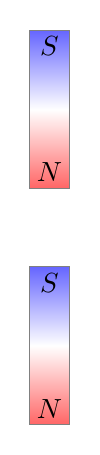
\begin{tikzpicture}
				\def\angle{90}% change this to rotate the magnet
				\begin{scope}[gray,text=black, rotate=\angle]
					\node[draw, left color=red!60,right color=blue!60,  middle color=white, 
					rotate=\angle, shading angle=90+\angle, minimum width=2cm, minimum height=0.5cm
					]
					at (0,0) (I) {};
					\node at (-0.8,0) {$N$};
					\node at (0.8,0) {$S$};
					
					\node[draw, left color=red!60,right color=blue!60,  middle color=white, 
					rotate=\angle, shading angle=90+\angle, minimum width=2cm, minimum height=0.5cm
					]
					at (-3,0) (I) {};
					\node at (-3.8,0) {$N$};
					\node at (-2.2,0) {$S$};
				\end{scope}
			\end{tikzpicture}
		\end{center}
		\captionof{figure}{Diagram of an attractive dipole.}
		\label{fig:attdip}
		
		\vfill\columnbreak
		
		\begin{center}
			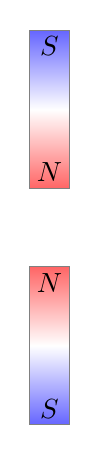
\begin{tikzpicture}
				\def\angle{90}% change this to rotate the magnet
				\begin{scope}[gray,text=black, rotate=\angle]
					\node[draw, left color=red!60,right color=blue!60,  middle color=white, 
					rotate=\angle, shading angle=90+\angle, minimum width=2cm, minimum height=0.5cm
					]
					at (0,0) (I) {};
					\node at (-0.8,0) {$N$};
					\node at (0.8,0) {$S$};
					
					\node[draw, left color=blue!60,right color=red!60,  middle color=white, 
					rotate=\angle, shading angle=90+\angle, minimum width=2cm, minimum height=0.5cm
					]
					at (-3,0) (I) {};
					\node at (-3.8,0) {$S$};
					\node at (-2.2,0) {$N$};
				\end{scope}
			\end{tikzpicture}
		\end{center}
		\captionof{figure}{Diagram of a repulsive dipole.}
		\label{fig:repdip}
	\end{multicols}
	
	\vspace{12pt}
	\begin{minipage}{\textwidth}
		\begin{center}
			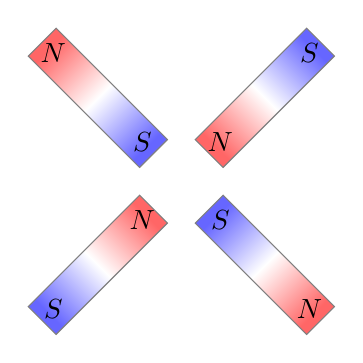
\begin{tikzpicture}
				\def\angle{45}% change this to rotate the magnet
				\begin{scope}[gray,text=black, rotate=\angle]
					\node[draw, left color=red!60,right color=blue!60,  middle color=white, 
					rotate=\angle, shading angle=90+\angle, minimum width=2cm, minimum height=0.5cm
					]
					at (0,0) (I) {};
					\node at (-0.8,0) {$N$};
					\node at (0.8,0) {$S$};
					
					\node[draw, left color=blue!60,right color=red!60,  middle color=white, 
					rotate=\angle, shading angle=90+\angle, minimum width=2cm, minimum height=0.5cm
					]
					at (-3,0) (I) {};
					\node at (-3.8,0) {$S$};
					\node at (-2.2,0) {$N$};
					
					\node[draw, left color=red!60,right color=blue!60,  middle color=white, 
					rotate=\angle, shading angle=\angle, minimum width=0.5cm, minimum height=2cm
					]
					at (-1.5,1.5) (I) {};
					\node at (-1.5,2.3) {$N$};
					\node at (-1.5,0.7) {$S$};
					
					\node[draw, left color=blue!60,right color=red!60,  middle color=white, 
					rotate=\angle, shading angle=\angle, minimum width=0.5cm, minimum height=2cm
					]
					at (-1.5,-1.5) (I) {};
					\node at (-1.5,-2.3) {$N$};
					\node at (-1.5,-0.7) {$S$};
				\end{scope}
			\end{tikzpicture}
			\captionof{figure}{Diagram of an attractive quadrupole.}
			\label{fig:quad}
		\end{center}
	\end{minipage}
	
	\section*{Analysis Questions}
	\begin{enumerate}
		%\item{How many tries did it take to get your magnet across the bench? Was it difficult?}
		%\item{Turn in your prediction vs observation sheets. You may turn in one per group, but make sure everyone's name is on it.}
		\item{How different were your predictions from observation? Be specific! For example, were there differences in size of the field loops?}
		\item{Magnetic fields are created by moving charges (current). How is it then that a bar magnet produces a magnetic field?}
		\item 
		\begin{enumerate}
			\item What are some similarities and differences between electric and magnetic dipoles? (For example: how are they constructed? what does the field look like? what are the two poles? etc...) 
			\item Is it possible to separate the charges in an electric dipole to form two separate ``monopoles''? What does the field of an electric monopole look like? Are magnetic monopoles possible? If so, what might the field of a magnetic monopole look like?
		\end{enumerate}
	\end{enumerate}
	
\end{document}
